\documentclass[12pt,a4paper]{article}

\usepackage[utf8]{inputenc}
\usepackage[T1]{fontenc}
\usepackage{polski}

\usepackage{amsthm}
\usepackage{amsmath}
\usepackage{amsfonts}
\usepackage{amssymb}
\usepackage{pgfplots}
\usepackage{tikz}
\usepackage{lmodern}	%fancy font
\usepackage{textcomp}

\usepackage{indentfirst}
\usepackage{graphicx}
\usepackage{caption}
\usepackage{subcaption}
\usepackage{siunitx}
\usepackage{here}


\setlength{\textheight}{24cm}
\setlength{\textwidth}{15.92cm}
\setlength{\footskip}{10mm}
\setlength{\oddsidemargin}{0mm}
\setlength{\evensidemargin}{0mm}
\setlength{\topmargin}{0mm}
\setlength{\headsep}{5mm}
\usepackage{tikz}
\usepackage{lmodern}	%fancy font
\usepackage{textcomp}

\usepackage{indentfirst}
\usepackage{graphicx}
\usepackage{caption}
\usepackage{subcaption}
\usepackage{siunitx}
\usepackage{here}
\usepackage[margin=1in]{geometry}% Just for this example
\setlength{\parindent}{0pt}% Just for this example
\setlength{\textheight}{24cm}
\setlength{\textwidth}{15.92cm}
\setlength{\footskip}{10mm}
\setlength{\oddsidemargin}{0mm}
\setlength{\evensidemargin}{0mm}
\setlength{\topmargin}{0mm}


\begin{document}

\begin{table}[]
\label{my-label}
\begin{tabular}{|p{7.5cm}|p{7.5cm}|}
\hline
									           					&                           \\

\includegraphics[height=3cm]{logo}             					& \textbf{Technika cyfrowa} \\ \hline
\multicolumn{1}{|l|}{\textbf{Temat ćwiczenia}} 					& \textbf{Numer ćwiczenia}  \\
\multicolumn{1}{|l|}{Minimalizacja i praktyczna realizacja złożonych funkcji logicznych}	& 2                         \\ \hline
\multicolumn{1}{|l|}{\textbf{Wykonawca}}       & \textbf{Ocena}            \\
\multicolumn{1}{|l|}{Miron Markowski}          &                           \\ \hline
\end{tabular}
\end{table}

\section{Cel ćwiczenia}


Zapoznanie się z zastosowaniem tablic Karnaugha do minimalizacji graficznej złożonych funkcji logicznych oraz zaprojektowanie w Multisimie układu cyfrowego zwiększającego o 1 trzybitową liczbę całkowitą oraz wyświetlacza siedmiosegmentowego.

\section{Przebieg ćwiczenia}

\subsection{układ cyfrowy zwiększający o jeden trzybitową nieujemną liczbę całkowitą}
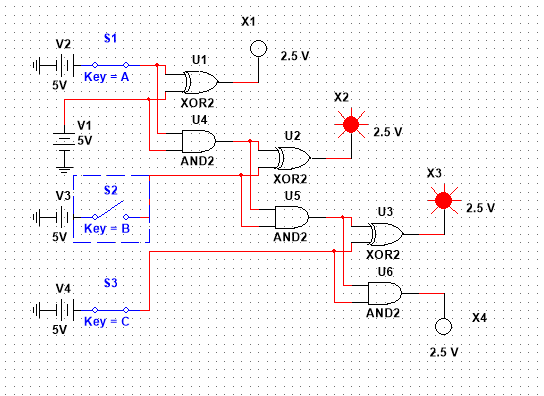
\includegraphics[width=\textwidth]{2a}
Układ składa się z 3 wejść reprezentujących 3 bitową liczbę całkowitą oraz 4 wyjść, z których to czwarte jest opcjonalne: reprezentuje ono flagę przeniesienia (carry flag). Najstarszy bit na wejściu i wyjściu znajduje się najniżej na wykresie.


\subsection{Minimalizacja funkcji metodą tablic Karnaugha}
Tutaj wstaw własną cudną minimalizację

\subsection{Transkoder czterobitowych cyfr}
Matkobosko
\end{document}